\documentclass{vldb}

\usepackage{graphicx}
\usepackage{balance}
\usepackage{booktabs}
\usepackage{multirow}
\usepackage{url}
\usepackage{newalg}
\usepackage{siunitx}
\usepackage{subfig}
\usepackage[pdftex,hypertexnames=true]{hyperref}

\newcommand{\dquote}[1]{``#1''}
\newcommand{\squote}[1]{`#1'}

\newdef{definition}{Definition}

\hyphenation{fra-mes}

\begin{document}

\thispagestyle{empty}
\pagestyle{empty}

\title{Data-driven Windows: The Theory and Practice of Frames}

\numberofauthors{1}

\author{%
\alignauthor
Michael Grossniklaus, David Maier, Sharmadha Moorty, Kristin Tufte\titlenote{Alphabetical order for the time being.}\\
       \affaddr{Computer Science Department}\\
       \affaddr{Portland State University}\\
       \affaddr{Portland, OR 97201, USA}\\
       \email{\{grossniklaus,maier,moorthy,tufte\}@cs.pdx.edu}
}



\maketitle

\begin{abstract}
Data Stream Management Systems (DSMS) segment potentially unbounded data streams into windows for processing. DSMS windows typically have the following three characteristics: they are defined on a timestamp or sequence-number attribute so that the window definition is independent of other data values in the stream; the window definitions are static and do not change in the course of query execution; and, finally, windows are filled with data from the stream over which the window is defined. These three aspects limit the power of traditional DSMS windows, while many applications have a need for more advanced windowing mechanisms. In this paper, we introduce \emph{frames}: a mechanism for defining dynamic, data-dependent windows that can be filled with data from other streams or even historical tables. We describe frame specification and implementation in the NiagaraST DSMS and show how frames can support sophisticated windows common to the needs of many applications including network monitoring and tracking vehicle traffic. 
\end{abstract}

\section{Introduction}
\label{sec:introduction}

Data Stream Management Systems (DSMS) have become commonplace in research and industry. DSMS process potentially unbounded data streams, producing results in real-time or near real-time. More recently, systems have been introduced that combine stream data with historical archives, providing the power of combining live stream data with historical archived data. The goal of DSMS is to give users \dquote{current} information about dynamic, unbounded data streams and, in the case of stream-archive systems, to put that current information in historical context.
 
To provide a \dquote{current} view over a stream, DSMS use windows. Windows segment the unbounded stream into finite subsets, which can be processed, aggregated over, selected on, and joined using variations on traditional DBMS operators. However, traditional DSMS windows have limitations that restrict their usefulness in certain applications. We see a need for new, more flexible and dynamic, windowing mechanisms.

Consider a network-monitoring application for analyzing the causes of poor router performance. The input data stream for this application consists of \texttt{loss\_rate} reports, which are issued from routers on a regular schedule. The application first detects extended periods of time during which a router has a high drop percentage (say, $> 0.3\%$). The application then uses the selected time periods to probe auxiliary data to shed light on the reason for the high loss. For example, we may discover that a high-loss period coincides with a large number of routing-table updates (BGP messages), which can be expensive to process. Consider supporting this application with traditional DSMS window functionality. Windows are typically defined over a timestamp attribute, based on a time range (window length) and an update frequency (slide). Such windows are less than ideal for this network-monitoring application for several reasons:
%
\begin{itemize}
\item They are defined in terms of a timestamp attribute; however the interval of interest (high-loss period) in this application depends on the loss rate reported by the router – a non-timestamp attribute in the stream.
\item Windows are filled with data from the stream over which the window is defined. However, to analyze the high-loss periods, we want to fill the window with data from an auxiliary stream.
\item The window definitions are static and do not change in the course of query execution. While the number of tuples per window may vary, the length of windows and their rate of production are fixed. In contrast, in the desired scenario above, windows adapt to patterns in the data: a window will only be produced if the high-loss condition occurs and the window will extend to the end of the high-loss period.
\end{itemize}

In this paper, we introduce frames, a mechanism for dynamic, data-dependent windows. As the name suggests, a frame defines only the boundaries of a window, that is, a start time and an end time. Frames segment data streams in an intrinsic, data-dependent way, based on the values in the data stream (e.g., \texttt{loss\_rate} in the example above), and can be filled with data from any stream (including the stream over which the frame is defined) or even historical data. Frames provide a sophisticated windowing mechanism that can support advanced monitoring applications and other scenarios that we describe later in the paper.

We have implemented a version of frames in NiagaraST~\cite{LTS+2008}, via a \emph{Frame} operator. In the implementation, we define frames as a period of time, with a given minimum duration, during which a predicate is satisfied. This definition satisfies the needs of the router-monitoring scenario described above. The implementation supports filling frames from an auxiliary stream via a \dquote{Between-Join}, handles disordered and missing data, and can take advantage of a regular data-delivery schedule for a stream, if such a schedule exists.

In this paper, we begin by discussing frame benefits, including differences between intrinsic and extrinsic segmentation, and then describe example scenarios that can benefit from frames. We present a general definition of frames, discuss our initial implementation of a Frame operator in the NiagaraST system---along with describing the kinds of frames it can handle---and follow with performance results. 

\section{Frame Benefits}
\label{sec:benefits}

As discussed in the introduction, windowing is ubiquitous in stream systems. Windowing was developed to deal with stateful and blocking operators, but current windowing mechanisms are limited in their ability to adapt to changing data streams and support segmentation that fits naturally to the particular phenomenon a user wants to examine. We discuss benefits of intrinsic segmentation, and the flexibility in filling frame in this section, followed in the next section by examples of applications that benefit from the intrinsic segmentation provided by frames. 

Frames support \emph{intrinsic} segmentation---the division of a stream based on some property of the data (thus segmentation will be different if data values are different). Furthermore, frames need not cover every element of a stream---they need only be reported for \dquote{interesting} segments. Traditional windowing mechanisms operate by extrinsic segmentation – the division of the stream is fixed in advance, and is independent of data values in the stream, other than a timestamp or sequence number. Typically, windows cover all elements of a stream and are emitted regularly, even during \dquote{uninteresting} periods. Of course, the output of a windowing operator can be sent through a filter to select out the notable window instances, however, the effort expended to construct the filtered-out windows is wasted. There are several reasons that the intrinsic segmentation provided by frames might be more beneficial than the extrinsic segmentation of normal windows:
%
\begin{itemize}
\item With intrinsic segmentation, the boundaries of segmentation adapt to the data, and might convey some information themselves, such as the duration of poor router performance.
\item Windows often serve to reduce data volumes to more manageable levels. However, fixed-size windows may not maximize information per window compared to an intrinsic segmentation that adapts to stream characteristics. For example, we might want to divide a network stream into periods of roughly equal payload volume, rather than by equal time intervals or numbers of packets. (The distinction is reminiscent of that between equi-depth and equi-width histograms~\cite{IP1995}.) 
\item Not every segment of the stream might be interesting – windows tend to put every tuple in at least one window; in the network router monitoring example, only periods of high loss are interesting, low loss is not interesting.
\end{itemize}

In addition to the benefits listed, frames derive from intrinsic segmentation that adapts to data in the stream, providing flexibility in how frames are filled. By \dquote{filling} frames, we mean associating a set of tuples with the frame, which tuples can then be the target of operations, such as aggregation or duplicate elimination. Such filling will typically be accomplished with a \dquote{between join} relating the timestamps of filling tuples to the bounds of the frame. 
%
\begin{itemize}
\item Frames may be filled from the same stream over which the frame was defined; this is most similar to windows. Note that the filling tuples need not be exactly the ones that contributed to frame detection. For example, once we have detected a high-loss period for a router, we might want to fill that frame with just the \dquote{very-high-loss} reports from the router ($> 1.5\%$) and count them.
\item Frames may be filled from another stream. This case corresponds to our router monitoring example, where the filler comes from the BGP message stream to the router.
\item Frames can be filled from stored data. For example, suppose we are defining frames using highway sensor data to select extended periods of slow traffic speed. We can fill such frames with stored data from the same time on previous days in order to understand whether this slow down is a normal occurrence or represents an unusual event.
\item Alternatively, frames themselves can be stored, and filled from later-arriving data. For example, we can hold on to the high-loss frames from the router, and fill them with Netflow records that are periodically dumped from the router, to get a sense of the number of different sessions using the router during the frame period.
\item Frames need not be filled at all, but might serve simply as alerts to trigger other actions, such as running network or router diagnostics.
\end{itemize}

Finally, we note that a single frame can be replicated and filled from several different sources, and that the filling tuples can be offset relative to the frame boundaries. For example, in filling a high-loss-period frame with BGP messages, we might include messages starting 30 seconds before the actual frame-start time.

\section{Use Cases}
\label{sec:usecases}

\begin{itemize}

\item Threshold Frames
\begin{itemize}
\item All segments where data value $>$ (equiv $<$) some threshold for some length of time
\item Maximal span 
\item No need for explicit start
\end{itemize}

\item Boundary Frames
\begin{itemize}
\item Frame on some boundary in the data--–i.e., frame every one meter of depth
\item What is the predicate?
\item How do we do this?
\item Max/min explicit, start explicit
\end{itemize}

\item Aggregate Frames
\begin{itemize}
\item $sum(vol) > threshold$
\item Minimal span
\item Minimal frames overlap; do need some sort of start info if we want to eliminate some of those frames 
\end{itemize}

\item Delta Frames
\begin{itemize}
\item $max(x) – min(x) > value$
\item start/minimal/maximal all seem undefined by predicate
\item idea is to use frames to capture regions of change
\end{itemize}

\item Michael’s Capture Trend Changes Idea

\end{itemize}

We present three examples scenarios in which frames may be useful and for which traditional DSMS windows will not suffice. 

\emph{Example 1--Vehicle-Traffic Monitoring:} In some cases, windowing can be seen as a form of approximation. Consider a stream of traffic speed and count data; the user wants to know the “current” speed for a particular location. Cumulative speed and vehicle count are reported every 20 seconds; however the 20-second data has high variance. A window can be used to smooth the jitteriness in the data. However, we observe that the length of window desired during high-volume traffic (rush hour) may be different than the length of window during low-volume (overnight) time periods. In the overnight period, one may wish to use a longer window to account for the lower flow of traffic and to avoid the window speed being biased by a single particularly fast (or slow) vehicle. Instead of windowing on time, one may wish to window based on the number of vehicles over which the average speed is recorded. Thus, we may want windows defined over the stream such that sum(\texttt{vehicle\_count}) $> 100$ for each window. In this example, a window with a fixed time period is a compromise and while a more desired and sophisticated window definition can be provided with frames.

\emph{Example 2--Freezer Temperature:} A commercial walk-in freezer contains a sensor that reports freezer temperature. One may wish to know periods of time greater than one minute during which the freezer temperature was too warm ($> 32$ degrees Fahrenheit). We could then correlate these periods with a stream of door open and close events to see if the door openings and closings are correlated with the high freezer temperatures. 

\emph{Example 3--Fine-grained Bursts:} A network-monitoring device produces reports of network usage every fifteen minutes. During certain 15-minute intervals, the reports show usage levels of only $3$-$4\%$ of total capacity but unusually high packet loss. Further inspection shows the presence of packet loss occurring during short-lived ($< 30$ second) bursts that saturate the network. We observe that it may be hard to know in advance the right granularity for monitoring; a technique like frames, which can dynamically adapt granularity, may be better for this application.

\section{Theory of Frames}
\label{sec:theory}

To give a formal specification of frames, we first define the framing of a data stream and then specify the functions that can be used to define a framing. We also describe how a framing can be used to fill frames with tuples from a stream. Finally, we introduce example of commonly used framings and describe how they can be expressed based on the given specification.

\begin{definition}
A \emph{data stream} $S$ is defined as an infinite sequence of tuples $S=[t_1, t_2, t_3, \ldots]$. All tuples of a data stream have the same schema. One attribute of the schema, the \emph{progressing attribute}, is distinguished as is defines the logical order of the tuples. The stream progresses in this attribute, i.e. if $A$ is this attribute, then for any $n$, there is an $i$ s.t. $t_i.A > n$. Note that while the presence of a progressing attribute implies a logical ordering, it does not require that the tuples within the stream are physically ordered.
\end{definition}

\subsection{Framing of a Data Stream}

For the purpose of this paper, we define the framing of a data stream incrementally by introducing the set of possible frames that is then restricted through local and global conditions to obtain the set of candidate and final frames, respectively.

\begin{definition}
The \emph{possible frames} $F_p(S)$ of a data stream $S$ are given by the infinite set of intervals (or framing) $F_p(S) = \{[s_1,e_1],[s_2,e_2],[s_3,e_3],\ldots\}$, such that $\forall [s,e] \in F_p(S): s,e \in \text{dom}(A)$, if $A$ is the progressing attribute and $\forall i < j: s_i \leq s_j \wedge s_i = s_j \Rightarrow e_i \neq e_j$.\footnote{The names $s_i$ and $e_i$ stand for start and end point, respectively.} Each interval $[s,e] \in F_p(S)$ defines an extent as a set of tuples $\{t | t \in S \wedge s \leq t.A < e \}$, where $A$ is the progressing attribute. Each interval $[s,e] \in F_p(S)$ has an \emph{extent} that is the set of tuples $\{t|t in S \wedge s \leq t.A < e\}$, where $A$ is the progressing attribute.
\end{definition}

Theoretically, all set of intervals that satisfy the conditions given in the definition are valid framings of a stream. In practice, however, it is useful to further constrain framings. We distinguish \emph{local} and \emph{global conditions} that can be applied to restrict which intervals are contained in a framing.

A local condition $p_l$ is a (conjunction of) predicates that can be checked individually  for each interval $[s,e]$ contained in the set of possible frames $F_p$. We distinguish data-de\-pen\-dent and data-independent predicates. For \emph{data-dependent predicates}, an expressions of the form $\textit{lhs} \theta \textit{rhs}$ has to hold for every tuple $t$ in $\text{extent}([s,e])$, where $\theta$ is a comparison operator, \textit{rhs} is a constant, and \textit{lhs} is a sub-expression built from arithmetic operators, aggregates, and universal quantification. The predicate $t.X > c$ for instance restricts the framing to intervals where the value of attribute $X$ of all contained tuples $t$ is consistently larger than a constant $c$. 

A \emph{data-independent predicate} guarantees the minimum (or maximum) duration of the interval. Duration can be expressed either in terms of the progressing attribute $A$ or the number of tuples contained in the $\text{extent}([s,e])$. In the former case, the second condition is given by $e.A - s.A \geq n$ (or $e.A - s.A \leq n$), while in the latter case, it is given by $|\text{extent}([s,e])| \geq n$ (or $|\text{extent}([s,e])| \leq n$), where $|\cdot|$ denotes set cardinality. The two conditions are used in a conjunction to form the local condition $p_l$ in the following definition.

\begin{definition}
The \emph{candidate frames} $F_c(S)$ of a data stream $S$ are those possible frames for which the local condition $p_l$ is true, i.e., $F_c(S) = \{[s,e] | [s,e] \in F_p(S) \wedge p_l([s,e]) \}$.
\end{definition}

Global conditions $p_g$ apply to all intervals in the set of candidate frames $F_c$, rather than to an individual interval. As a global condition, we can require that all intervals are either \emph{minimal} or \emph{maximal}. For example, a set of candidate frames obtained by the threshold predicate above is not guaranteed to report a unique set of intervals as for every interval that satisfies the predicate all sub-intervals down to individual tuples could be reported. In this case, requiring the framing to be maximal ensures that only non-overlapping intervals of maximal length are reported.

Another global condition that guides the selection of candidate frames is whether a set of intervals is \emph{saturated} or \emph{drained}. A set of frames is saturated if it satisfies all conditions and there is no candidate frame that can be added to it without violating a condition (set maximality). A final framing is drained if it satisfies all conditions and there is no frame that can be removed from it without violating a condition (set minimality).

\begin{definition}
The \emph{final frames} $F_f(S)$ of a data stream $S$ are the candidate frames for which all global conditions $p_g^1, \ldots, p_g^n$ are true, i.e., $F_f(S) = \{[s,e] | [s,e] \in F_c(S) \wedge [s,e] \in F_c(S) \Leftrightarrow \bigwedge_{1 \leq i \leq n} p_g^i(F_f(S))\}$.
\end{definition}

\subsection{Properties of Framings}

Depending on the local and global conditions chosen for a framing, we can observe different framing schemes that describe how a stream is segmented. Figure~\ref{fig:framing-schemes} summarizes important framing schemes.

\begin{figure}[htb]
   \centering
   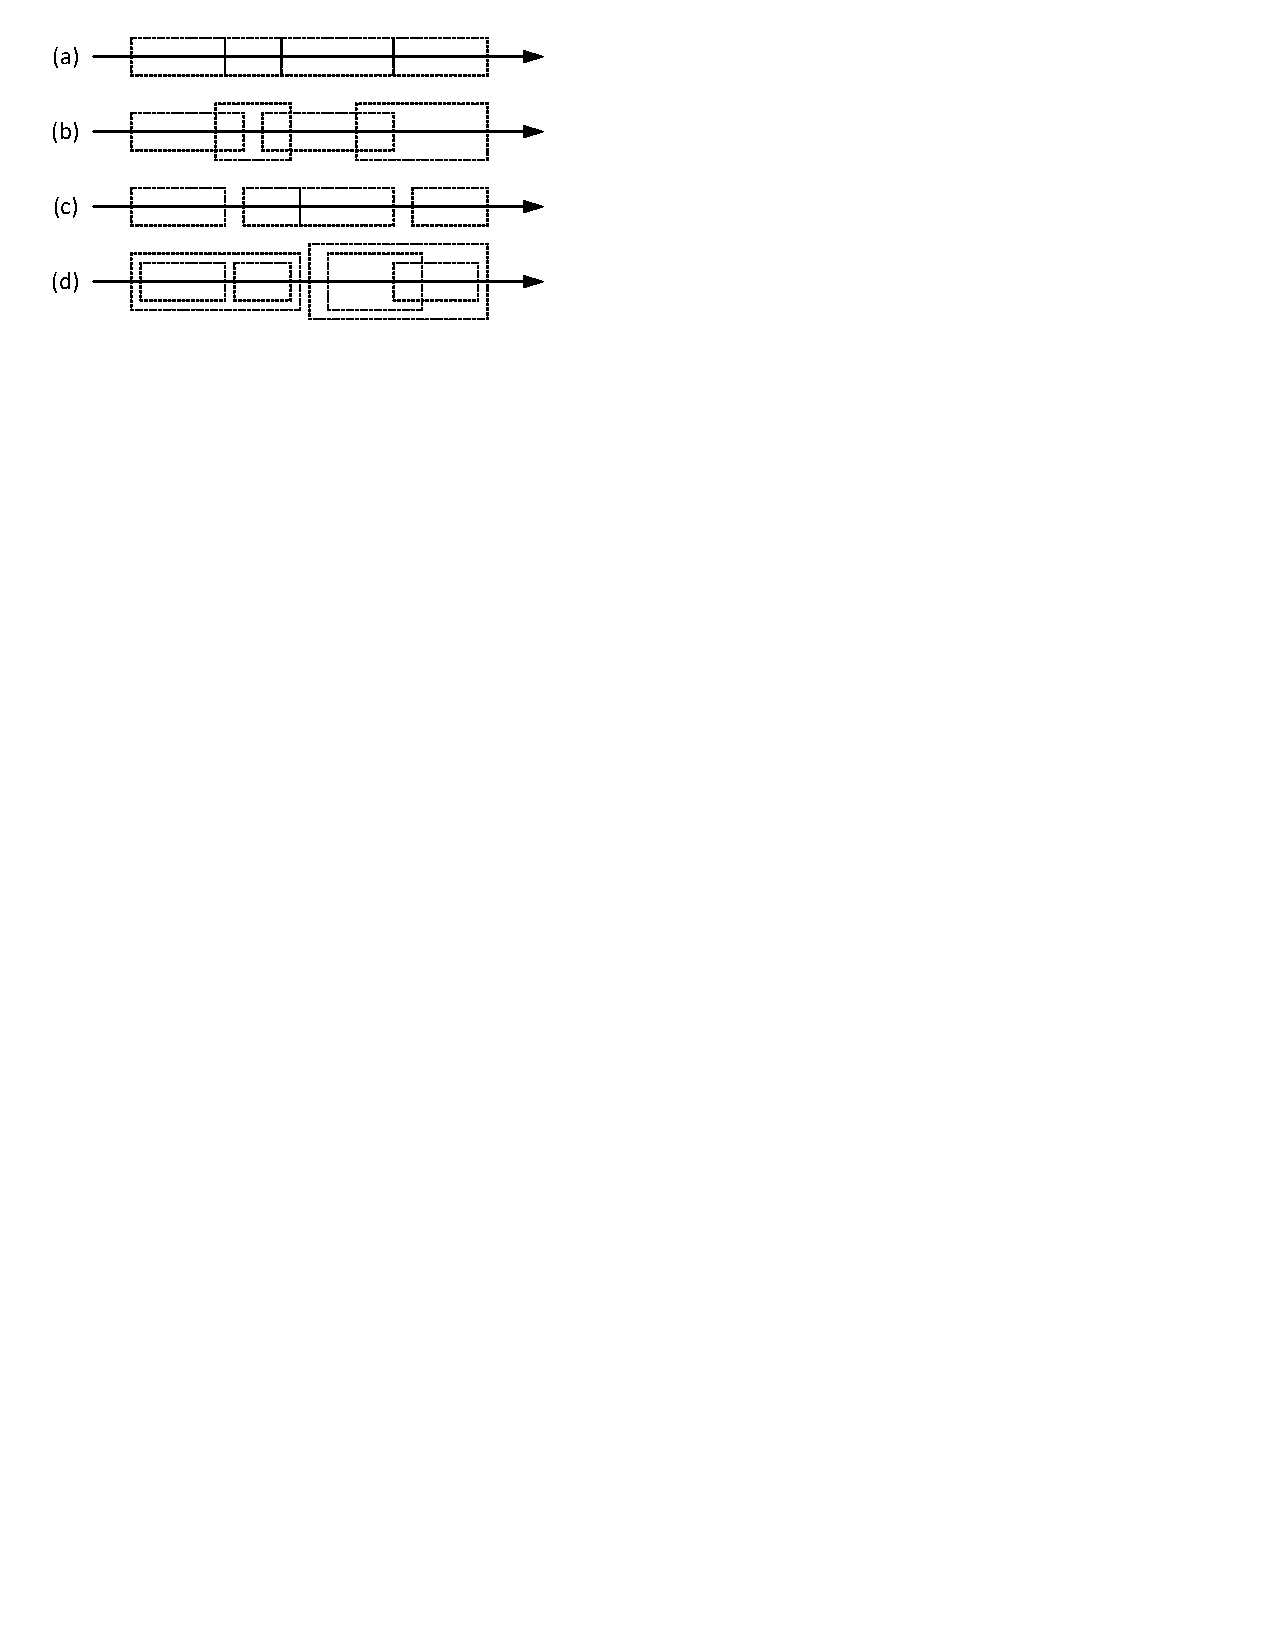
\includegraphics[width=.9\columnwidth]{figures/framing-schemes}
   \caption{Different framing schemes}
   \label{fig:framing-schemes}
\end{figure}

\begin{description}

\item[Partition.] Each interval $[s_i,e_i]$ begins where the previous frame $[s_{i-1},e_{i-1}]$ ended, i.e., $s_i = e_{i-1}$. Note that this segmentation of the stream is similar to tumbling windows. However, intervals still vary in length, whereas windows are of fixed length, either in terms of time or tuples.

\item[Cover.] $\forall a \in \text{dom}(A): \exists [s_i,e_i] \in F: s_i < a \leq e_i$, where $A$ is the progressing attribute, i.e., $s_i \leq e_{i-1}$. Note that this segmentation of the stream is similar to sliding windows. However, neither the slide offset nor the interval length is fixed. A special case of this segmentation is the case where intervals overlap by fixed value $c$, i.e., $s_i = e_{i-1}-c$. We will refer to this stream segmentation as adjacent. Another special case are advancing intervals, where we require that $b_i < b_{i+1} \wedge e_i < e_{i+1}$.

\item[Disjoint.] $\forall [s_i,e_i] \in F: \not\exists [s_j,e_j] \in F: s_j \leq s_i \leq e_j \vee s_j \leq e_i \leq e_j$, i.e., $s_i \geq e_{i-1}$. Note that with this segmentation it is possible that some values $a \in \text{dom}(A)$, where $A$ is the progressing attribute, are not contained in any intervals.

\item[Unconstrained.]

\end{description}

\subsection{Examples}

Coming back to the use cases presented in Section~\ref{sec:usecases}, we now describe a series of types of frames that address the requirements outlined earlier. We also discuss how each of these types can be specified within the framework introduced in this section.

\textbf{Threshold Frames:} This type of frame reports periods of the stream where the value of a user-defined attribute a is greater (or smaller) than a given threshold value $x$. As a consequence, this type of frame does not partition or cover the stream. It is defined by the frame predicate $a>x$ (or $a<x$). The start point is data dependent, i.e., a frame starts as soon as the predicate is true. The span is maximal in the sense that the frame keeps growing as long as the predicate holds true. An example of use for this type of frame is to report high-loss periods.

\textbf{Boundary Frames:} Boundary frames segment the stream whenever the value of a user-specified attribute crosses a (multiple of) a given boundary $x$. This type of frames partitions the stream. The frame predicate for the $n^\text{th}$ frame is given by $a < nx$, whereas the data-dependent starting point is defined by $a > (n-1)x$. The span is minimal. Note that if attribute a is a progressing attribute, this equivalent to windows.

\textbf{Delta Frames:} This type of frame monitors a user-specified attribute a of the tuples in the data stream. A frame is emitted whenever the delta between the minimum and maximum value of this attribute becomes greater than a predefined value $x$. This type of frame partitions the stream. The frame predicate can therefore be given as $max⁡(a)-min⁡(a) < x$. The frame starting point is the end point of the previous frame and the span of the frames is maximal.

\textbf{Aggregate Frames:} This type of frames monitor a predicate over an aggregation of an attribute. Aggregate frames segment the stream. The frame predicate is given by $f_\text{aggr}(a) \ \theta \ x$, where $f_\text{aggr}$ is an aggregation function and $\theta$ is a comparison operator. The start point of aggregate frames is the end point of the previous frame and its span can either be minimal or maximal, depending on the desired reporting scheme. An example of this type of frame is segmenting on the maximum sum of dye mass.

\subsubsection{Notes}

\textbf{Threshold and Boundary Frames}
\begin{itemize}
\item the union of overlapping candidate frames is a candidate frame
\end{itemize}

\textbf{Boundary Frames}
\begin{itemize}
\item any tuple is in some candidate frame
\item full coverage comes from the fact that any single tuple frame satisfies the predicate
\end{itemize}

\textbf{Delta and Aggregate Frames}

Below \emph{minimal} is used for predicates that require the delta or aggregate to be greater than a constant, whereas \emph{maximal} is used when the delta or aggregate needs to be smaller than a constant.
\begin{itemize}
\item a minimal/maximal frame from a starting point $T_1$ cannot properly contain a minimal/maximal frame from starting point $T_2$, where $T_1 > T_2$
\item without minimal duration, these framings have coverage using a drained framing of minimal/maximal frames (note that this framing is unique as the first frame needs to be picked which then defines the starting point of the next frame, etc.)
\end{itemize}

\subsection{Framing Function}

A framing as defined in the previous section is a function that returns a sequence of frame intervals for a given data stream. However, in order to process the data stream as it progresses, we require that this function can be computed incrementally, based on the previously computed frame intervals and the next tuple of the stream.

\begin{definition}
A \emph{framing function} $f(F_{i-1}, C_{i-1}, t_i ) \rightarrow (F_i, C_i)$ applies the $i^\text{th}$ tuple to the current framing $F_{i-1}$ and returns a new framing $F_i$. The framing $F_i$ is an extension of the framing $F_{i-1}$, i.e., $F_{i-1} \subseteq F_i$. $C_{i-1}$ and $C_i$ denote the respective state before and after application of f for the $i^\text{th}$ tuple.
\end{definition}

$C$ manages both the internal state of the framing function and the list of frames that are currently being processed, i.e., the open frames. For every arriving tuple, the framing function needs to decide whether (a) to open a new frame, (b) update an existing frame, or (c) close and emit a frame. In the latter case, the frame is removed from state $C$ and inserted into the framing $F$. Depending on the framing scheme, all of these actions can be applied once or multiple times. In order to control the behavior of a framing function, we have identified the following frame properties.

We conclude this subsection by outlining an example template of a framing function that generates partitioning frames.\\

\begin{algorithm}{Partition}{F_{in},C_{in},t,p} %→(F_{out},C_{out})
   f_{old} \= [s_{old},e_{old}] | [s_{old},e_{old}] \in C_{in} \\
   \begin{IF}{p(t,C_{in})}
      F_{out} \= F_{in} \\
      f_{new} \= [s_{old},ts(t)]
   \ELSE
      F_{out} \= F_{in} \cup \{ f_{old} \} \\
      f_{new} \= [ts(t),ts(t)]
   \end{IF}\\
   C_{out} \= C_{in} \backslash f_{old} \cup \{ f_{new} \} \\
   \RETURN (F_{out}, C_{out})
\end{algorithm}

The function template begins by extracting the current frame from the state $C$. Note that there is only one open frame in the state as this template follows the partition scheme. On line 2, the predicate is evaluated. If it still holds, the current frame is extended (lines 3 and 4). If not, the current frame is emitted (line 5) and a new frame is opened (line 6). Finally, the state is updated to reflect the updated or new frame (line 7). The function $ts(\cdot)$ is used to return the value of the progressing attribute of a tuple.

\subsection{Filling Frames}

Once a framing of a stream has been defined in terms of a sequence of intervals, it can be used to fill frames. A framing that has computed based on one stream can be used to produce frames of that stream or any other stream. A frame filling $\hat{F}$ is given as a set of tuple sequences $\hat{F} = \{ \langle t_1, t_2, \ldots t_i \rangle, \ldots \langle t_{n-j}, \ldots t_{n-1}, t_n \rangle \}$.

\begin{definition}
A \emph{frame filling} is defined by a function $f: (S' \times g(F) \times Q) \rightarrow \hat{F}$, where $S'$ is the data stream furnishing the tuples, $F$ is the framing, and $Q$ is a query.
\end{definition}

The function $g(\cdot)$ allows intervals in the framing to be modified. For example, the function could be used to extend or reduce the lengths of intervals by a fixed amount. In particular, it can be used to produce adjacent frames. In contrast, the query $Q$ defines a subset of the tuples that fall into the interval of the frame, or performs aggregation.

\section{Implementation}
\label{sec:implementation}

\section{Evaluation}
\label{sec:evaluation}

\begin{figure*}[t]
\centering
\subfloat[][Unprocessed Data]{
   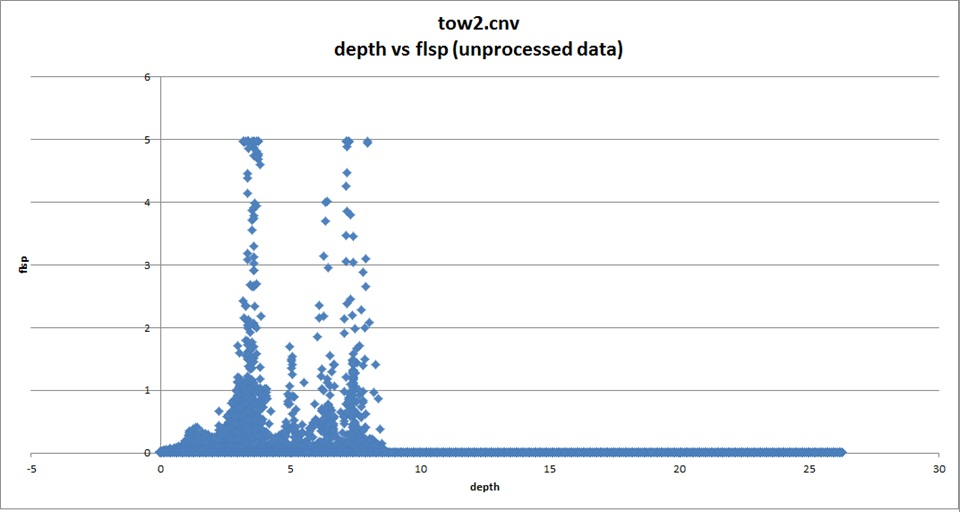
\includegraphics[width=.313\textwidth]{figures/tow2_cnv_original1000}
   \label{fig:eval-tow02-original}
}
\subfloat[][Windowed Data]{
   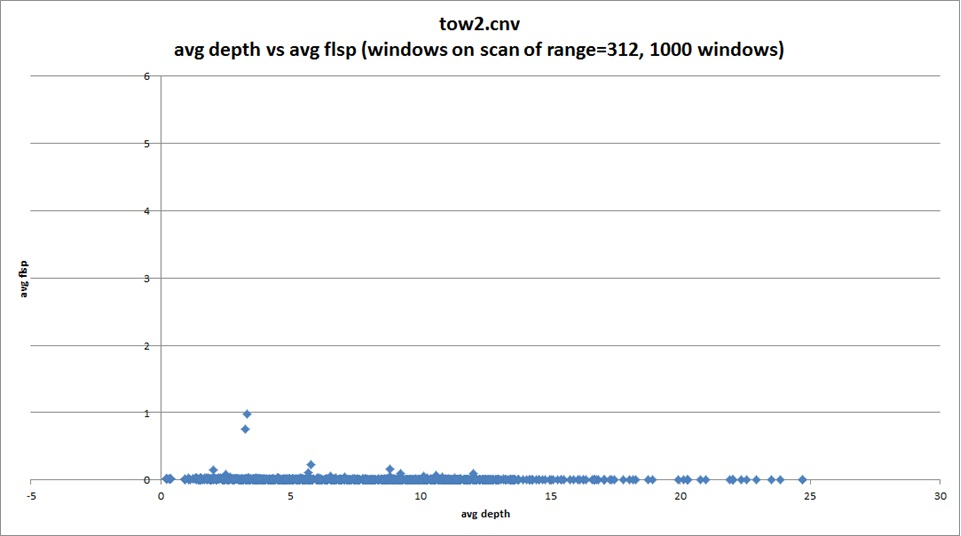
\includegraphics[width=.313\textwidth]{figures/tow2_cnv_windows1000}
   \label{fig:eval-tow02-windows}
}
\subfloat[][Framed Data]{
   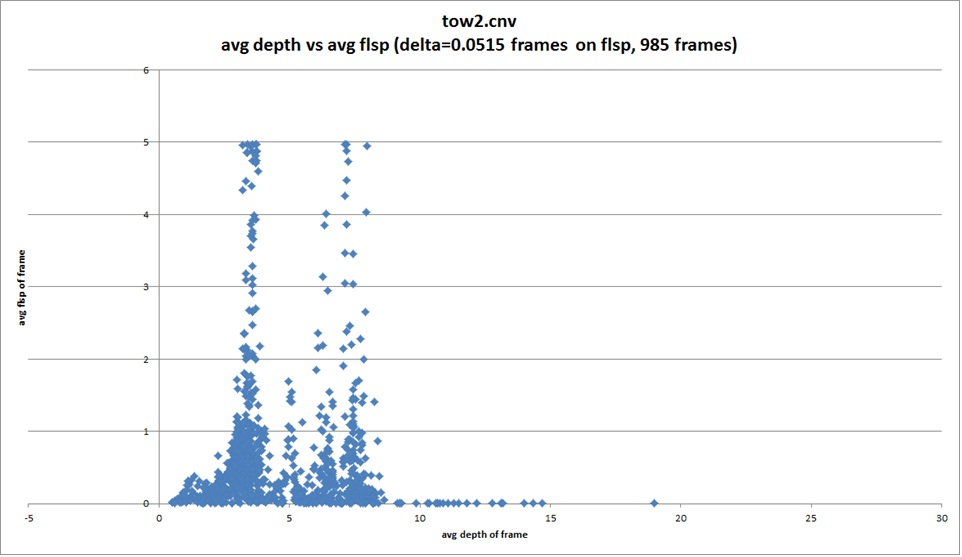
\includegraphics[width=.313\textwidth]{figures/tow2_cnv_frames1000}
   \label{fig:eval-tow02-frames}
}
\caption{Comparison of original versus windowed and framed data sets}
\label{fig:eval-tow02-all}
\end{figure*}

\begin{figure}[htb]
   \centering
   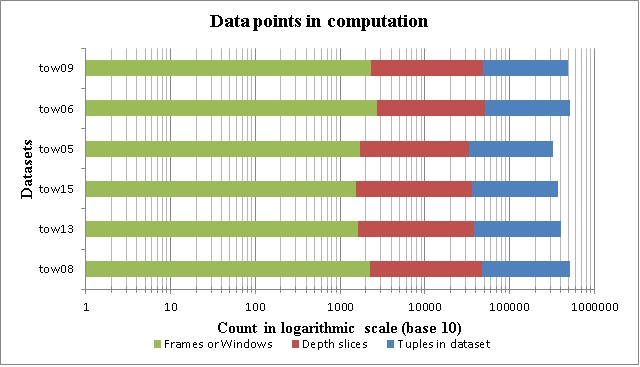
\includegraphics[width=.99\columnwidth]{figures/datapointsInComputation}
   \caption{Data point in computation}
   \label{fig:eval-datapoints}
\end{figure}

\begin{figure}[tb]
   \centering
   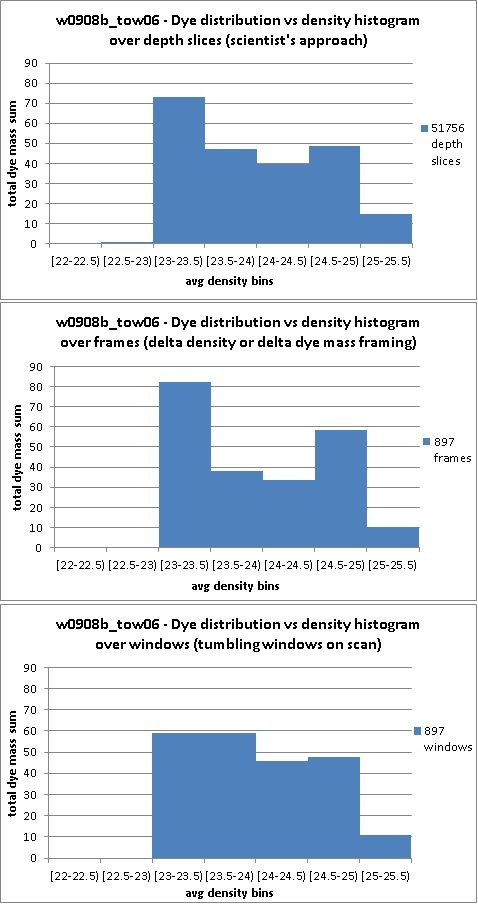
\includegraphics[width=.99\columnwidth]{figures/histogram_tow06}
   \caption{Histogram tow06}
   \label{fig:eval-histogram-tow06}
\end{figure}

\begin{figure}[tb]
   \centering
   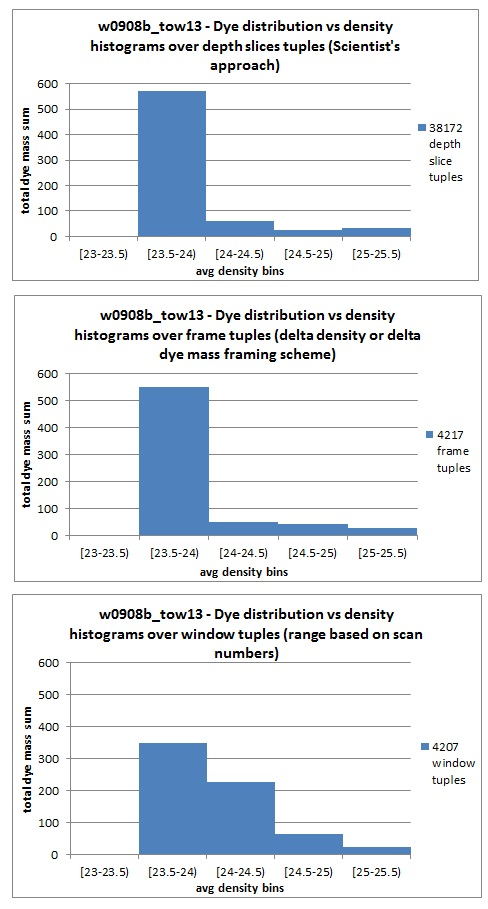
\includegraphics[width=.99\columnwidth]{figures/histogram_tow13}
   \caption{Histogram tow13}
   \label{fig:eval-histogram-tow13}
\end{figure}

\begin{figure}[htb]
   \centering
   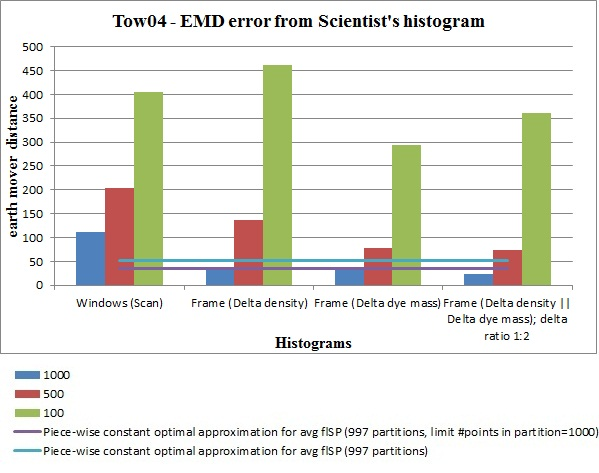
\includegraphics[width=.99\columnwidth]{figures/tow04_results}
   \caption{EMD error from Scientist's histogram (tow04)}
   \label{fig:eval-emd-error-tow04}
\end{figure}

\begin{figure}[htb]
   \centering
   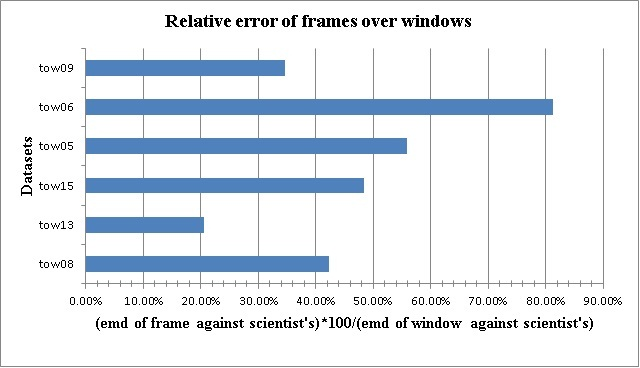
\includegraphics[width=.99\columnwidth]{figures/relativeErrorFramesOverWindows_6datasets}
   \caption{Relative error of frames over windows}
   \label{fig:eval-relative-error}
\end{figure}

\begin{figure}[htb]
   \centering
   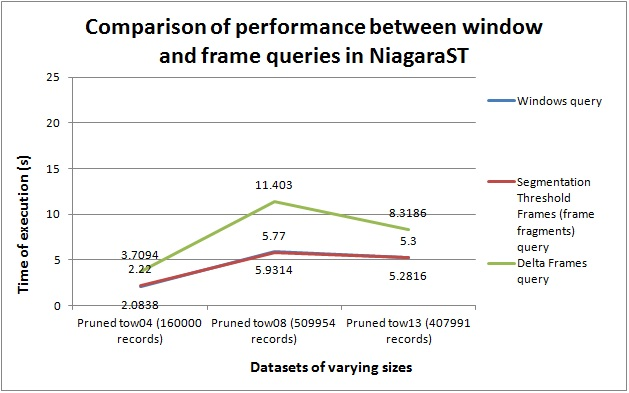
\includegraphics[width=.99\columnwidth]{figures/performance_analysis}
   \caption{Comparison of performance between window and frame queries in NiagaraST}
   \label{fig:eval-performance-analysis}
\end{figure}


\section{Related Work}
\label{sec:relatedwork}

\section{Conclusions}
\label{sec:conclusion}

\balance

\section{Acknowledgments}
The authors thank Ted Johnson for the sustained-loss router example, which actually started us on this line of work. The IPTV example also comes from conversations with him. James Whiteneck and Rafael Fern{\'a}ndez helped with early implementations and examination of frames. Oregon State University’s \dquote{Team Florescin} collected the dye data: Murray Levine, Steve Pierce and Brandy Cervantes.

This work is supported in part by National Science Foundation grant IIS-0917349. Michael Grossniklaus's participation is funded by the Swiss National Science Foundation (SNSF) grant number PA00P2\_131452.

% REFERENCES

\nocite{*}

\bibliographystyle{abbrv}
\bibliography{vldb2013}

% APPENDIX
\begin{appendix}

\section{Cutting Room Floor}

Note that some of the local properties imply global properties. For example, requiring intervals to be maximal at the local level will always lead to a disjoint framing scheme as overlapping intervals can be combined into a single interval. Similarly, certain constraints on the starting points of interval will also directly yield a certain framing scheme. For example, to specify an adjacent segmentation, the starting point condition would be defined as $s_i=e_{i-1}$, while the condition $s_i=e_{i-1}+1$ yields a partitioning of the stream. As a consequence, care has to be taken in order not to specify conflicting conditions.

Furthermore, we allowing multiple possible interval starting points using a complex expression together with a non-overlapping framing scheme, the situation may arise where a starting point occurs before the ending point of the preceding interval. We use policies to indicate which condition will be violated by the framing if such a situation arises. There are three possibilities.
\begin{enumerate}
\item Close and report the preceding interval: This policy will lead to a framing that possibly violates the local condition defined by the predicate.
\item Drop and suppress the previous interval: This policy possibly leads to false negatives in terms of the local condition defined by the predicate. It will also possibly violate the global condition of a covering (or partitioning) framing scheme.
\end{enumerate}

\textbf{Continue the previous interval:} This policy does not violate any of the local conditions, but possibly violates a requirement to generate a non-overlapping framing scheme.

\section{Frame Definition (Dave/CIDR)}
\label{sec:theory-cidr}

A frame is a dynamic, data-dependent mechanism for computing window boundaries based on data values in a stream. As its name suggests, a frame represents only the beginning and end of a window extent and not does specify the data used to \dquote{fill} the window. Typically a frame will define the start timestamp and end timestamp of a window.

At an abstract level, a \emph{framing scheme} $F$ is a mapping from a sequence of elements of type $T$ to a set of frames, each of which bounds a portion of the sequence: $$F: Seq(T) \rightarrow \{(\text{fs}: Time, \text{fe}: Time)\}$$ Here \squote{$\text{fs}$} is for \dquote{frameStart} and \squote{$\text{fe}$} for \dquote{frameEnd}. We assume each frame element has an attribute drawn from a totally ordered domain, such as timestamps or sequence numbers. For the moment, we do not constrain F. Thus it can depend in any manner on the values of elements and their arrangement.

Consider a sequence $S$ with elements of type $\langle Time, Temperature \rangle$: 
\begin{center}
$\langle 1, 30 \rangle, \langle 2, 31 \rangle, \langle 3, 33 \rangle, \langle 4,34 \rangle, \langle 5, 30 \rangle,$ \\ 
$ \langle 6, 34 \rangle, \langle 7, 33 \rangle, \langle 8, 34 \rangle, \langle 9, 35 \rangle, \langle 10, 32 \rangle$
\end{center}
Some example framing schemes, along with their results on $S$:

$F_1$. (locally) maximal periods where Temperature $> 32$.  $F_1(S) = \{(\text{fs}: 3, \text{fe}: 4), (\text{fs}: 6, \text{fe}: 9)\}$. Note that $(\text{fs}: 7, \text{fe}: 9)$ is not in $F_1(S)$, because it is not maximal---$(\text{fs}: 6, \text{fe}; 9)$ contains it.

$F_2$. (globally) maximum period where Temperature $> 32$. $F_2(S) = \{(\text{fs}: 6, \text{fe}: 9)\}$. Note that $(\text{fs}: 3, \text{fe}: 4)$ is not in $F_2(S)$, since it does not have maximum duration.

$F_3$. maximal periods where Temperature is increasing over at least three time units. $F_3(S) = \{(\text{fs}: 1, \text{fe}: 4), (\text{fs}: 7, \text{fe}: 9)\}$.

In these particular examples, the result set will not contain overlapping frames, but in general overlap is allowed.

Not every framing scheme will be realizable in a stream setting where the sequence of elements is presented over time and we want to detect and report frames incrementally. Framing schemes $F_1$ and $F_3$ above can be computed incrementally---the existence of a frame and its bounds can be determined once the next element after the frame end has been seen. For framing scheme $F_2$ however, the existence of a frame is not definite until all the input has been seen, which could be arbitrarily in the future. Hence, we could only report a result for $F_2$ over a stream if the stream ends. Thus, we are interested in classes of framing schemes that can be evaluated incrementally over streams.

Our own prototyping efforts are based on framing schemes that arise naturally in the monitoring of network or vehicular traffic, two application areas on which we have focused. Our framing schemes are specified as a maximal interval over which some predicate holds, possibly with a minimum duration. Thus, $F_1$ above is expressible in our specification, as would be $F_1'$ that also requires that the period must be at least 3 time units long. Because our frame specifications mandate maximality, frame instances will not overlap. For example, suppose our specification requires \texttt{loss\_rate} $> 0.3\%$ for at least 5 minutes. Then we could not have two frame instances $(\text{fs}: 10:13, \text{fe}: 10:20)$ and $(\text{fs}: 10:18, \text{fe}: 10:23)$, because $(\text{fs}: 10:13, \text{fe}: 10:23)$ must be a period where the \texttt{loss\_rate} condition holds continuously, and it subsumes either of the other frames. However, for other styles of frame specification, such as based on event density, maximality might not exclude overlap.

\section{Implementation Considerations (CIDR)}
\label{sec:considerations-cidr}

Many issues arise in moving from the abstract notion of framing schemes to an implementation in a DSMS. 

\emph{Long Frames:} Consider again the router-monitoring example, high-loss periods could extend for minutes or tens of minutes depending on the cause of the problem. It does not seem appropriate to wait until the end of the frame to notify the user; instead, the user should be notified as soon as the start and end of the frame is detected. It may make sense to periodically report the extension of the frame between those two points, but probably not every time it is extended.

\emph{Disorder:} Another pragmatic issue is stream disorder. We assume that a framing scheme is relative to a logical order induced by some timestamp-like attribute. If physical delivery order is different from this logical order, we may need additional information, such as punctuation or an expected delivery schedule, to know that a frame has definitely been detected.

\emph{Scheduled vs. Non-scheduled Data:} Data in some streams arrives on a regular schedule. For example, router \texttt{loss\_rate} reports are sent at specified intervals and the highway-sensor reports arrive every 20 seconds. In contrast, a freezer sensor may report temperature only on temperature change and trades in a stock market ticker have no schedule. If the stream has a reporting schedule, frames can be detected based on the presence of a set of expected tuples; if there is no reporting schedule, one must wait for punctuation~\cite{TMS+2003} to determine frame existence. 

\emph{Missing Data:} Missing data can be detected if there is a reporting schedule. (If not, missing data might not be detected or may require a sophisticated algorithm for detection.) Missing data must be addressed in the frame specification. For example, in the router example, should a missing data value be considered a high-loss or low-loss record? It turns out that the answer may depend on context---a missing data item in the middle of a period of high loss is likely to be a high loss record that got dropped due to network saturation; however, a missing record during a time of low loss should not be assumed to be a high-loss record. In general, if the stream has a reporting schedule, consideration must be given to how missing data is interpreted as it will directly affect the extents of the frames. In Figure~\ref{fig:missing-tuples}, tuples A and B are missing. If A is true and B is false, there are 3 and 4 true tuples in a row. If both are true there are 8 true tuples in a row.

\begin{figure}[htb]
   \centering
   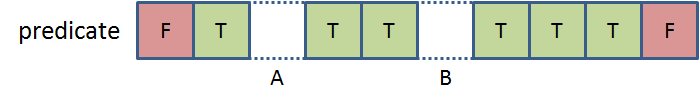
\includegraphics[width=.99\columnwidth]{figures/missing-tuples}
   \caption{Tuples A and B are missing}
   \label{fig:missing-tuples}
\end{figure}
 
\emph{Groupwise Frames:} So far we have discussed framing sche\-mes being applied over the entirety of a stream. However, frames can also be defined \dquote{groupwise}---that is, the framing scheme is applied per substream defined by a group-by attribute, and frame instances are tagged with the value of that attribute. A consequence of groupwise treatment is that frames for different groups will have different start and end times; in contrast with time-based windows where the window start and end times are consistent across groups.

\emph{Data Semantics:} Data arrives as tuples with timestamps, however the tuple data can be interpreted in different ways. Given a tuple \emph{t}, representing freezer temperature with data value \emph{d} and timestamp \emph{ts}, how do you interpret that tuple? Does \emph{t} represent a point-in-time event at time \emph{ts}? Or does \emph{t} represent an event beginning at time \emph{ts} and continuing until the next event? Different interpretations lead to different frame boundaries and may affect the implementation. Addition of start and end timestamps to each tuple as is done in CEDR~\cite{GHA+2007} may help.
 
\emph{Uniqueness of Time:} We require that timestamps on tuples be unique. Multiple readings at one timestamp may occur for reasons including multiple sensors contributing to one logical reading or an error. In either case, preprocessing can be done—such as to aggregate together multiple sensors or to clean the data—to resolve the issue. This cleaning or aggregation should happen before the data is sent to the frame-processing operators, though the specification of those operators must be mindful   of preprocessing procedures, as they can affect frame existence and duration. 
Frame Extent: There is some subtlety in how the framing scheme picks the starts and ends of frames. A liberal framing scheme might apply to the freezer example, wherein we would like regions when the freezer temperature was possibly $>$ 32 degrees, and hence the frame extends from the last sub-freezing report all the way to the next report at or below 32. In contrast, a more conservative scheme might apply to the router example, wherein we might want only regions where we know for sure that the loss rate is high.

\section{Related Work (CIDR)}
\section{sec:relatedwork-cidr}

Past research on data-driven windows includes work on predicate-windows by Ghanem~\emph{et al.}~\cite{GAE2006,GEL+2009}. Tuples enter into and expire from a predicate-window depending on whether they satisfy the predicate associated with the window. Predicate windows have features in common with frames that the extent of a window can depend on values of the stream elements. Some predicate windows may be expressible as framing schemes and vice-versa. However, there are two key differences. First, a predicate window instance does not necessarily correspond to a contiguous range over the input stream. Second, the contents of a window is determined by applying a predicate individually to each stream element that is \dquote{live} at a particular time \emph{t}, and generally does not depend on the arrangement of those elements. (The predicate windows approach posits a \emph{correlation} attribute CORAttr, such that a later tuple $e_2$ with the same CORAttr value as a previous tuple $e_1$ is assumed to be an update of $e_1$. In this instance, a later tuple can affect the inclusion of an earlier tuple.) 

Various pattern-matching methodologies have been proposed previously for stream-processing systems, including SASE+~\cite{ADG+2008}, Cayuga~\cite{BDG+2007} and AFAs~\cite{CGM2010}. Other pattern-matching work that is not stream-based includes SQL-TS, an extension to SQL that supports searching for complex patterns in database systems~\cite{SZZ+2004} and S-OLAP, a flavor of online analytical processing system that supports grouping and aggregation of data based on patterns~\cite{CKL+2010}. Pattern-matching techniques for streams or relations could be the basis for a framing scheme, with a frame corresponding to a span of events that match the pattern. Additional conditions of maximality of matches or non-overlap might be imposed in addition. There would need to be extensions to the techniques to deal with out-of order and missing data, and to exploit reporting schedules.

In contrast to their window counterparts, frames are adaptive. Adaptive mechanisms and systems have been proposed in the past for stream management systems, including CAPE~\cite{RDS+2004}, StreaMon~\cite{BW2004} and AdaptWID~\cite{LTD+2008} adaptive query processing in general. Some of these techniques adapt to stream contents in terms of tuple density or data-distribution properties. Frames, by comparison, adapt based on properties of the data and its clustering.

\section{NiagaraST Implementation (CIDR)}
\label{sec:implementation-cidr}

As a test framework, we have implemented one version of frames in the NiagaraST~\cite{LMT+2005a} stream processing system. NiagaraST is a data stream processing system written in Java and developed at Portland State University. NiagaraST is based on the Niagara~\cite{NDM+2001} system from the University of Wisconsin-Madison In this prototype, the frame specification consists of two parts---a predicate and a (time) duration: \dquote{Predicate $P$ holds for duration at least $D$}. $P$ is a tuple-wise predicate over the stream. $D$ can be expressed as a number of tuples or minimum time interval. The implementation supports frames such as those required for the router-monitoring example. A possible frame specification for the router example is: \dquote{\texttt{tuple.loss\_rate} $> 0.3\%$ for at least 3 reports}. We take the maximal period satisfying the condition. In this example, if there were 5 consecutive high-loss reports in a row, we would report it as a single frame instance (rather than three instances of length 3).

We have implemented two operators in NiagaraST to support frame processing: an Apply operator to process the predicate P and a Frame operator to interpret the predicate sequences, looking for ones that meet the duration condition D. More specifically, Apply applies P to each input tuple and appends a true or false value to it. These tuples are fed to the Frame operator, which uses the duration D to form frames.

The frame operator takes parameters to specify the minimum frame duration, a missing data predicate, and existence of reporting schedule. Frame output consists of a unique frame id, frame start and end times, and a flag to indicate if the frame is partial or final. A partial frame is an early indication that $D$ has been satisfied and is still true. A final frame indicates that $D$ is no longer true and the frame start and end times are final. All data is assumed to have a timestamp attribute, but tuples are not assumed to arrive in order; and the input stream may or may not have a known reporting schedule. The methods for detecting a frame depend on how and when data arrives. If the data arrives on a schedule, the Frame operator takes advantage of that schedule and uses it to output frames as they are detected. If there is no reporting schedule, the operator waits for Punctuation to finalize frame detection. Punctuation is used to deal with disordered data.

Missing data is handled with two conditions. First, we require that any frame begin with a known value that satisfies the predicate $P$; that is, a frame cannot begin with a missing value. Second, the frame specification specifies whether missing data values should be considered as satisfying the predicate $P$ or not. We plan to extend this simple specification to allow slightly more complex patterns. For example, in the router example, missing values should be assumed to satisfy the predicate (that is, be high-loss records) if they are in the midst of other high-loss records and should be assumed to not satisfy the predicate in other cases.
 
To handle the \dquote{Long Frame} problem mentioned in Section~\ref{sec:considerations}, we support breaking a frame into a sequence of \emph{fragments}. We emit an initial fragment when were a certain a new frame instance will occur: we have seen a sequence of tuples that satisfy P of at least duration D, and we know (via a reporting schedule or punctuation) that this sequence cannot merge with an earlier frame nor be divided by a non-satisfying tuple. As additional tuples arrive that extend the sequence, the Frame operator will periodically output incremental fragments, with a final fragment once the end time of the frame is known. The different fragment types are indicated by a flag in the output tuples of Frame.

We expect that fragmenting frames may have benefits for latency and memory use when filling frames. A frame may be filled via a join with the filling stream and the resulting tuples will likely be further aggregated. For example, high-loss frames in the router example can be joined on time with a BGP message stream, and then passed to an aggregate to perform a count of the different message types. For a long frame without fragmentation, the join process would not start until the end of the frame is detected; resulting in latency and the need to buffer the BGP stream at the join. In contrast, if the frame is delivered as fragments, each fragment can be joined with the BGP stream as received, allowing the matching tuples to be purged and the result tuples to be forwarded to the aggregate operator for processing.

\section{Evaluation (CIDR)}
\label{sec:evaluation-cidr}

We evaluated the performance of our frame implementation in the NiagaraST system over various sizes of input data and with various frame specifications selected specifications to vary the density and length of frames. We also compared our frame implementation with a frame-like window query that produces similar results and evaluated the latency impacts of various frame fragment sizes. 

All experiments were run on a 3.00 GHz Intel Core2 Duo 3.00 GHz Processor with 4GB of memory running Windows 7 Enterprise and running Java Runtime Environment Version 6 (1.6.0\_21), with the \texttt{–server} option, and with 1.5 GB allocated memory to the JVM. For all queries, we use a data set of traffic records. The data is from approximately 600 sensors on the Portland-Vancouver metropolitan area freeways that report traffic speed and count every 20 seconds.

\begin{figure}[htb]
   \centering
   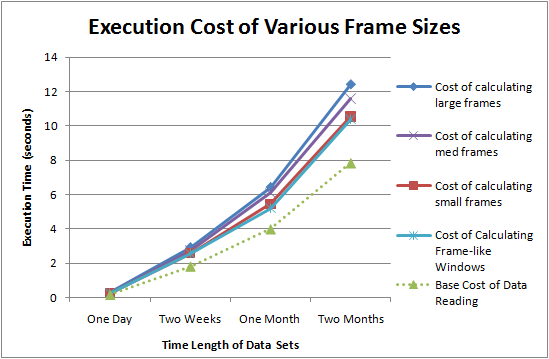
\includegraphics[width=.99\columnwidth]{figures/eval-experiment-1}
   \caption{Experiment 1: Frame performance over various data sets and frame specifications}
   \label{fig:eval-experiment-1}
\end{figure}

For the first experiment, shown in Figure~\ref{fig:eval-experiment-1}, we ran three frame specifications over four data sets---ranging from 1 day of traffic data ($4320$ reports) to two months of data ($267840$ reports). We measured performance of frame length, short, medium and long in order to test different frame densities. Note that by density of frames, we are referring to the total \% of tuples in all frames, not the density of the tuples within the frames themselves. Table~\ref{tab:frame-specs} lists the frame specifications as well as the average frame length and percentage of tuples in frames, a measure of frame density. Figure~\ref{fig:eval-experiment-1} shows the performance of the framing queries for these specifications over the various data sets. The base cost of reading the data is indicated as a dotted line. As the size of the dataset increases the cost of computing frames also increases. This is based on our initial implementation and we believe the cost can be brought down by optimizing the algorithm.

\begin{table}[htb]
\centering
\caption{Frame Specifications used in Experiments 1 \& 2}
\begin{tabular}{cS[table-format=4.0]S[table-format=4.0]S[table-format=1.5]}
\toprule
\multicolumn{1}{c}{\textbf{Frame}} & \multicolumn{1}{c}{\textbf{\# of}} &
\multicolumn{1}{c}{\textbf{Avg}} & \multicolumn{1}{c}{\textbf{\# of}} \\
\multicolumn{1}{c}{\textbf{Specification}} & \multicolumn{1}{c}{\textbf{Frames}} &
\multicolumn{1}{c}{\textbf{Frames}} & \multicolumn{1}{c}{\textbf{Tuples}} \\
\midrule
Short (Speed $\leq 30$)    &  302  &  38 & 0.04284 \\
Medium (Speed $\geq 50$)	& 3071  &  39 & 0.44719 \\
Long (Speed $\geq 30$)     &  866  & 278 & 0.89885 \\
\bottomrule
\end{tabular}
\label{tab:frame-specs}
\end{table}

We can create a result similar to a frame result using traditional NiagaraST windows. The basic idea is logically illustrated in three steps: first, create sliding windows of length equal to the minimum frame duration and slide by each time step; second, aggregate over those windows with a predicate derived from the frame predicate; and finally select windows that match the frame predicate. While this process will not create the same output as frames, it does create a similar result. Further processing is required to coalesce windows to create the maximal window as opposed to producing many smaller windows. The cost of calculating a frame-like window is indicated in Figure~\ref{fig:eval-experiment-1}.

For our third experiment we used a modified join query to test performance of detecting and filling frames. To fill frames, we joined the frame operator output with a traffic stream to fill in the framed time periods and aggregated vehicle speed. We used a special Between-Join that allowed punctuation to free blocked tuples to the aggregating operator and process frame fragments individually. We also tested the impact of frame fragment sizes on the latency of the results, as indicated in Figure~\ref{fig:eval-fragments} above. When frame lengths are short and/or punctuations are frequent, the fragment size makes little difference. However, when frame fragments are long, having short punctuation can provide a substantial benefit as seen in Figure~\ref{fig:eval-fragments}.

\begin{figure}[htb]
   \centering
   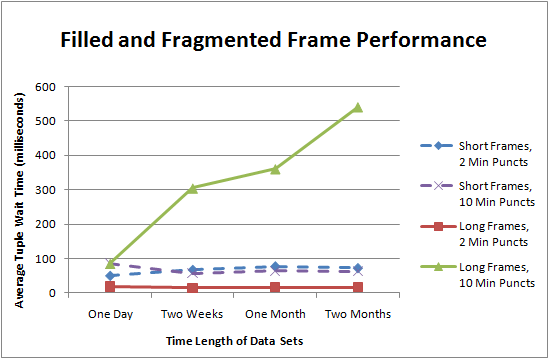
\includegraphics[width=.99\columnwidth]{figures/eval-fragments}
   \caption{Frame Fragment Size and Latency Performance}
   \label{fig:eval-fragments}
\end{figure}

\section{Future Work (CIDR)}
\label{sec:futurework}

We believe frames are a valuable addition to the windowing capabilities of DSMS. Their computational requirements are similar to those for fixed-period windows, but they can express data in segments and over predicates in ways not expressible by windows.

One of our main interests for future work is other styles of frame specification. In particular, frames may be defined on density criteria. For example, we might be interested in periods where vehicle count at a highway sensor exceeds 30 vehicles per minute. One issue with density-defined frames is that maximality of duration might not be the most useful choice. Consider a 2-minute period with 90 vehicles followed by a 2-minute period with 30 vehicles. Do we want to report the full 4-minute period, or would reporting just the initial 2-minute period be more informative? Scan statistics~\cite{GPW2009} may provide guidance here. Scan statistics consider the local density of events in a sequence or region, and can help calculate the likelihood that a particular density occurs by chance given an a priori global distribution. Thus, in our traffic example, it may be possible to determine whether 90 vehicles in 2 minutes is more unusual than 120 vehicles in 4 minutes and select a frame on that basis. Scan statistics might also be used directly to specify frames. We may want to report a frame of duration d spanning k tuples if the probability of such a cluster occurring by chance (assuming some distribution) is .05 or less. 

A second area we have been investigating is frames with both spatial and temporal extent~\cite{WTB+2010}, such as stretches of highway at least 2 miles long that have reduced speeds for at least 30 minutes. One interesting issue here is that maximality does not guarantee non-overlap. There might be a 3-mile stretch with slow traffic for 30 minutes that overlaps a 2-mile stretch with slow traffic for 45 minutes. While we do not intend to prohibit overlapping frames outright, we may want some prioritization mechanism so that we do not over-report the same underlying phenomenon.
 
\end{appendix}

\end{document}
